% ЕМТ 2022, V клас — точен LaTeX препис от официалните файлове в Klasirane.com.
% Условия: https://klasirane.com/api/competitions/EMT/All/2022/5%20%D0%BA%D0%BB/probs
% SHA-256 (условия): 499a808c3f700dcf207e1f5aec0ee389402430e5522c4814a35aee11abab4d2d
% Решения: https://klasirane.com/api/competitions/EMT/All/2022/5%20%D0%BA%D0%BB/sol
% SHA-256 (решения): 31ba05123fb689c5d6cc9018cfbd4f48f74a77ed046c93317f8ce9a7789bd7e7
% Точковите оценки, правописът, формулировките и видимите печатни особености са запазени от източника.
% Фигурата е неизменен изрез от официалния PDF с условията, изобразен с 4 пиксела на PDF точка.

Задача 5.1. Парк има форма на триъгълник $ABC$, страните на който са алеи. По алеите пътят от $A$ до $B$ през $C$ е 646 m, пътят от $B$ до $C$ през $A$ е 561 m, а пътят от $C$ до $A$ през $B$ е 595 m.

Във върховете $A$, $B$, $C$ и покрай алеите на парка засадили дървета така, че разстоянието между всеки две съседни дървета е $n$ метра, където $n$ естествено число, по-голямо от 1.

А) Колко метра е дълга всяка от алеите $AB$, $BC$ и $CA$?

Б) Колко дървета са засадили?

В) Един ден градинар обиколил алеите в посока $A\to B\to C\to A$, като поставял къщичка за птици на всяко четвърто дърво по пътя си. На другия ден той обиколил алеите в посока $A\to C\to B\to A$ и на всяко пето дърво по пътя си поставял къщичка за птици, ако там вече нямало. И двата дни броенето започвал с дървото в $A$. Колко къщички е поставил той?

Решение. а) По условие $AB+BC=595$, $BC+CA=646$, $CA+AB=561$. Като съберем трите равенства, получаваме $2(AB+BC+CA)=1802$, откъдето $AB+BC+CA=901$. Тогава $AB=901-646=255$, $BC=595-255=340$, $CA=646-340=306$.

б) Числото $n$ е по-голям от 1 делител на 340, 306 и 255. Тъй като $\operatorname{НОД}(340,306,255)=17$, то $n=17$. Дърветата са $901:17=53$.

в) Ако номерираме 53-те дървета в посока $A\to B\to C\to A$ с номерата 1, 2, 3 и т.н., първия ден градинарят е поставил къщички на всички дървета с кратен на 4 номер. Те са 13 дървета.

На втория ден той е преброил дървото в $A$, дърво 53, 52, 51 и е поставил къщичка на дърво 50, след това на дърво 45 и т.н. на дърветата с номер, кратен на 5. Тези дървета са 10. От тях той е пропуснал дърветата с номер, кратен на $\operatorname{НОК}(4;5)=20$, на които вече има къщичка; това са 2 дървета с номера 20 и 40. Общо къщичките са $13+10-2=21$.

Критерии за оценяване.

а) 2 точки; за намиране на обиколката – 1 т.

б) 2 точки; за намиране на НОД – 1 т.

в) 2 точки.

Задача 5.2. Четирицифреното число $M$ има следните свойства:

• числото $M$ е кратно на 9;

• ако разменим местата на цифрите на единиците и хилядите в $M$, се получава четирицифрено число, което е кратно на 5;

• ако разменим местата на цифрите на десетиците и стотиците в $M$, се получава число, което е кратно на 4;

• ако разменим местата на цифрите на стотиците и хилядите в $M$, се получава четирицифрено число, което е кратно на 11.

а) На колко може да е равно числото $M$? Посочете всички възможности.

б) Ако числото $M$ е равно на произведението на три последователни естествени числа, намерете сбора на тези три числа.

Решение. Нека числото е $M=\overline{abcd}$. От условието, че $\overline{dbca}$ и $\overline{bacd}$ са четирицифрени числа следва, че цифрите $d$ и $b$ не са равни на 0.

От $5\mid\overline{dbca}$ следва, че $a=5$ (като първа цифра, $a$ не е 0).

От $4\mid\overline{5cbd}$ следва, че $4\mid\overline{bd}$. (1)

От $9\mid\overline{5bcd}$ следва, че $9\mid 5+b+c+d$. Но $5+b+c+d$ не надхвърля 32, следователно $5+b+c+d=9$, 18 или 27. (2)

От $11\mid\overline{b5cd}$ следва, че 11 дели разликата на $b+c$ и $5+d$. Тъй като $b+c-(5+d)$ е най-много $2\cdot9-(5+1)=12$, а $5+d-(b+c)$ е най-много $5+9-(1+0)=13$, то разликата на $b+c$ и $5+d$ е 0 или 11.

Ако разликата на $b+c$ и $5+d$ е 11, сборът на четирите цифри е нечетен и по-голям от 11; от (2) следва, че този сбор е 27. Тогава $b+c$ и $5+d$ (в някакъв ред) са $(27-11):2=8$ и $(27+11):2=19$, но последното равенство е невъзможно.

Следователно $b+c=5+d$, сборът на четирите цифри е четен и от (2) следва, че този сбор е 18, т.е. $b+c=d+5=9$. Тогава $d=4$ и от (1) $b=2$, 4, 6 или 8.

При $b=2$ получаваме $c=7$ и $M=5274$.

При $b=4$ получаваме $c=5$ и $M=5454$.

При $b=6$ получаваме $c=3$ и $M=5634$.

При $b=8$ получаваме $c=1$ и $M=5814$.

б) От четирите получени възможности за $M$ ще потърсим числото, което може да се представи като произведение на три последователни естествени числа.

Имаме $5274=2\cdot3\cdot3\cdot293$, $5454=2\cdot3\cdot3\cdot3\cdot101$ и $5634=2\cdot3\cdot3\cdot313$; и в трите има прост делител, който е твърде голям, за да е изпълнено условието. Остава $5814=2\cdot3\cdot3\cdot17\cdot19=17\cdot18\cdot19$. Търсеният сбор е $17+18+19=54$.

Критерии за оценяване. а) 4 точки; б) за разлагане на множители 1 т.; за вярно намерен отговор (независимо по какъв начин) 2 точки.

Задача 5.3. Магистрала между градовете $A$ и $B$ е дълга 999 km. На всеки километър е поставена по една табела, от едната страна на която пише колко километра остават до $B$, а от другата страна пише на колко километра е табелата от $A$.

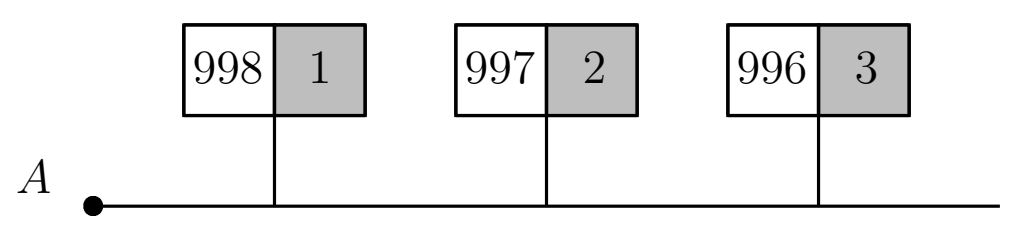
\includegraphics[max width=0.48\textwidth, alt={Първите три километрови табели от A към B}, center]{assets/5-3-road-signs.png}

а) Една табела е късметлийска, ако за записа на двете числа върху нея са използвани едни и същи две цифри. Например, табелите $(9/990)$ и $(818/181)$ са късметлийски. Колко късметлийски табели има по пътя?

б) Една табела е специална, ако записаните на нея числа имат най-малко общо кратно 7800. На колко километра от $A$ се намира първата специална табела?

Решение. а) Сборът на числата на всяка табела е 999. Късметлийските табели са от следните видове:

• $\overline{aaa}$, $\overline{bbb}$, където $a+b=9$ и $a$ е от 1 до 8; общо 8 табели;

• $\overline{aab}$, $\overline{bba}$, където $a+b=9$ и $a$ е от 0 до 9; общо 10 табели;

• $\overline{aba}$, $\overline{bab}$, където $a+b=9$ и $a$ е от 0 до 9; общо 10 табели;

• $\overline{baa}$, $\overline{abb}$, където $a+b=9$ и $a$ е от 0 до 9; общо 10 табели.

(В това броене при $a=0$ или $b=0$ получаваме двойките 009 и 990; 090 и 909; 099 и 900, които съответстват на табелите (9, 990); (90, 909); (99, 900).)

Получихме, че късметлийските табели са $8+3\cdot10=38$.

б) Търсим числа $a$ и $b$, за които $a+b=999$ и $\operatorname{НОК}(a;b)=7800=2^3\cdot3\cdot5^2\cdot13$.

Тъй като сборът на числата е нечетен, едното от тях е четно, а другото е нечетно; нека $a$ е четно. В разлагането на $a$ участва $2^3$.

В $\operatorname{НОК}(a;b)$ участва множител 3 и сборът на числата се дели на 3; следователно в разлагането и на двете числа има множител 3.

В $\operatorname{НОК}(a;b)$ участва $5^2$, а сборът на числата не се дели на 5; следователно в разлагането на точно едно от числата участва $5^2$. По същия начин е ясно, че в разлагането на точно едно от числата има множител 13.

Като вземем предвид, че $a<999$, възможните случаи са:

$a=2^3\cdot3\cdot5^2=600$, $b=3\cdot13=39$, но сборът не е 999;

$a=2^3\cdot3\cdot13=312$, $b=3\cdot5^2=75$, но сборът не е 999;

$a=2^3\cdot3=24$, $b=3\cdot5^2\cdot13=975$, сборът е 999.

Специалната табела е на 24 km от $A$.

Критерии за оценяване. а) 4 точки; б) 3 точки.

Задача 5.4. а) Иво има 3 карти $\boxed{\mathrm A}$, 3 карти $\boxed{\mathrm B}$ и 3 карти $\boxed{\mathrm C}$. Той подрежда деветте карти в редица.

Разстояние между две карти в редицата наричаме броя на картите между тях. За всеки две еднакви карти Иво записва разстоянието между тях.

Например, в редицата $\boxed{\mathrm A}\boxed{\mathrm B}\boxed{\mathrm C}\boxed{\mathrm A}\boxed{\mathrm A}\boxed{\mathrm B}\boxed{\mathrm C}\boxed{\mathrm B}\boxed{\mathrm C}$ разстоянията между картите с буквата $A$ са 0, 2 и 3, между картите с буквата $B$ са 1, 3 и 5, а между картите с буквата $C$ са 1, 3 и 5. Различните разстояния са 0, 1, 2, 3 и 5 и са пет на брой.

Най-много колко различни разстояния между еднакви карти може да получи Иво?

б) Най-много колко различни разстояния между еднакви карти може да получи Иво, ако подреди в редица 4 карти $\boxed{\mathrm A}$, 4 карти $\boxed{\mathrm B}$ и 4 карти $\boxed{\mathrm C}$?

Решение. а) Възможните разстояния между две карти са от 0 до 7; общо 8. Ще докажем, че винаги поне едно от тези осем разстояния не се среща.

Да допуснем, че се срещат и осемте разстояния. Разстояние 7 може да се появи само между първата и последната карта в редицата, така че първата и последната карта са с една и съща буква; нека е $A$. Разстоянието 6 може да се появи само между първата и осмата карта или между втората и деветата. Тъй като първата и деветата са с $A$, то втората или осмата също е $A$. Тогава картите са $AXXXXXXAA$ или $AAXXXXXXA$, където $X$ е $B$ или $C$. Но и в двата случая няма как да се появи разстояние 5, защото разстоянията между картите с $A$ са 0, 6 и 7, а между картите с $B$ или $C$ не са повече от 4.

Следователно винаги поне едно от разстоянията от 0 до 7 не се реализира. Броят на различните разстояния е най-много 7.

Пример за редица, в която се срещат 7 различни разстояния, е
$$
\boxed{\mathrm A}\boxed{\mathrm B}\boxed{\mathrm B}\boxed{\mathrm C}\boxed{\mathrm A}\boxed{\mathrm C}\boxed{\mathrm C}\boxed{\mathrm B}\boxed{\mathrm A}.
$$

б) Възможните разстояния между две карти са от 0 до 10; общо 11. Два примера, в които те се реализират, са следните:
$$
\boxed{\mathrm A}\boxed{\mathrm A}\boxed{\mathrm C}\boxed{\mathrm B}\boxed{\mathrm C}\boxed{\mathrm B}\boxed{\mathrm C}\boxed{\mathrm B}\boxed{\mathrm C}\boxed{\mathrm A}\boxed{\mathrm B}\boxed{\mathrm A}
$$
и
$$
\boxed{\mathrm A}\boxed{\mathrm A}\boxed{\mathrm C}\boxed{\mathrm B}\boxed{\mathrm B}\boxed{\mathrm C}\boxed{\mathrm B}\boxed{\mathrm C}\boxed{\mathrm C}\boxed{\mathrm A}\boxed{\mathrm B}\boxed{\mathrm A}.
$$

Критерии за оценяване. а) 5 точки; за оценка – 3 т., за пример 2 т. б) 2 точки за посочен верен пример.
